\documentclass[12pt,a4paper]{article}
% Estilo compartido para informes. Compilar con LuaLaTeX desde tp1/.
\usepackage[spanish,es-nodecimaldot]{babel}
\usepackage{fontspec}
\setmainfont{Montserrat-Medium.ttf}[
  Path=../assets/fonts/,
  BoldFont=Montserrat-Bold.ttf,
  ItalicFont=Montserrat-MediumItalic.ttf]
\usepackage[a4paper,margin=2.5cm,headheight=16pt]{geometry}
\usepackage{xcolor,graphicx,booktabs,tabularx}
\usepackage{float}
\usepackage{titlesec,fancyhdr,enumitem,caption}
\usepackage{ragged2e}
\usepackage{hyperref}
\definecolor{verde}{HTML}{1D4036}
\definecolor{bronce}{HTML}{D38129}
\definecolor{rosa}{HTML}{D88E77}
\definecolor{calido}{HTML}{EFE4D8}
\definecolor{grafito}{HTML}{1D1D1D}
\hypersetup{colorlinks=true,linkcolor=verde,urlcolor=verde,
  pdftitle={TP1 - Instalación de máquinas virtuales},pdfsubject={Cyberseguridad}}
\AtBeginDocument{\color{grafito}\RaggedRight\fontsize{12}{14.4}\selectfont}
\setlength{\parindent}{0pt}
\setlength{\parskip}{7pt}
\setlist[itemize]{leftmargin=*,itemsep=7pt,topsep=4pt}
\setlist[enumerate]{leftmargin=*,itemsep=6pt}
\titleformat{\section}{\color{verde}\bfseries\fontsize{18}{21.6}\selectfont}{\thesection}{0.65em}{}
\titleformat{\subsection}{\color{verde}\bfseries\large}{\thesubsection}{0.65em}{}
\titleformat{\subsubsection}{\color{verde}\bfseries}{\thesubsubsection}{0.65em}{}
\titlespacing*{\section}{0pt}{16pt}{8pt}
\titlespacing*{\subsection}{0pt}{12pt}{5pt}
\titlespacing*{\subsubsection}{0pt}{10pt}{4pt}
\setcounter{tocdepth}{2}
\pagestyle{fancy}
\fancyhf{}
\fancyhead[L]{\small\color{verde}FCEFyN | UNC}
\fancyhead[R]{\small\color{verde}\materia\ · TP \numeroTP}
\fancyfoot[L]{\scriptsize Informe de laboratorio}
\fancyfoot[R]{\small\thepage}
\renewcommand{\headrulewidth}{0.4pt}
\captionsetup{font=small,labelfont=bf,justification=raggedright,singlelinecheck=false,hypcap=false}
\newcommand{\pendiente}[1]{\par{\small\color{verde}\textbf{Por completar.} #1\par}}
% Si falta una captura se muestra un espacio reservado; no impide compilar.
\newcommand{\captura}[2]{%
  \par\smallskip\begingroup\centering
  \IfFileExists{figuras/#1}{%
    \includegraphics[width=\linewidth,height=5cm,keepaspectratio]{figuras/#1}%
  }{%
    \setlength{\fboxsep}{10pt}%
    \fcolorbox{bronce}{calido}{\parbox[c][1.25cm][c]{\dimexpr\linewidth-2\fboxsep-2\fboxrule\relax}{%
      \centering\small Captura pendiente\par\texttt{\detokenize{#1}}}}%
  }%
  \captionof{figure}{#2}\par\endgroup\smallskip
}

\usepackage{xurl}

\newcommand{\materia}{Cyberseguridad}
\newcommand{\numeroTP}{17}
\newcommand{\tituloTP}{Investigación de incidentes de seguridad}
\newcommand{\estudiante}{Brigido Tomas Andres}
\newcommand{\legajo}{38481096}
\newcommand{\carrera}{ICOMP}
\newcommand{\docente}{Javier A. Jorge}


% Metadatos específicos del TP17 y capturas en img/.
\hypersetup{pdftitle={TP17 - Investigación de incidentes de seguridad},linkcolor=black,urlcolor=black,citecolor=black}
\renewcommand{\captura}[2]{%
  \begin{figure}[H]
    \centering
    \IfFileExists{img/#1}{%
      \includegraphics[width=0.85\linewidth,height=6cm,keepaspectratio]{img/#1}%
    }{%
      \setlength{\fboxsep}{10pt}%
      \fcolorbox{bronce}{calido}{\parbox[c][1.1cm][c]{0.85\linewidth}{%
        \centering\small Captura pendiente\par\texttt{\detokenize{#1}}}}%
    }%
    \caption{#2}
  \end{figure}
}

\usepackage{caption}
\captionsetup{justification=centering}
\begin{document}
\hypersetup{pageanchor=false}
\begin{titlepage}
  
\includegraphics[width=8cm]{../assets/logo-fcefyn-2026.png}
  \vspace{1cm}

  {\color{verde}\small UNIVERSIDAD NACIONAL DE CÓRDOBA\par}
  \vspace{2.1cm}
  {\color{bronce}\bfseries\large TRABAJO PRÁCTICO \numeroTP\par}
  \vspace{0.45cm}
  {\color{verde}\bfseries\fontsize{32}{38.4}\selectfont Investigación de\\incidentes de seguridad\par}
  \vspace{0.3cm}
{\small Análisis de registros con Security Onion\par}
\vspace{0.35cm}
  {\large \materia\par}
  \vspace{0.8cm}
  {\color{bronce}\rule{2.7cm}{2pt}\par}
  \vfill
  \renewcommand{\arraystretch}{1.45}
  \begin{tabular}{@{}p{3.2cm}p{10cm}@{}}
    Estudiante & \estudiante \\
    Legajo & \legajo \\
    Carrera & \carrera \\
    Docente & \docente \\
  \end{tabular}
  \vfill
  {\small Córdoba, Argentina\par}
\end{titlepage}
\hypersetup{pageanchor=true}

\tableofcontents
\vspace{1cm}
\newpage


% Cada pregunta deja un espacio editable para una respuesta breve.
\newcommand{\pregunta}[1]{\par{\sloppy\textbf{#1}\par}\nopagebreak\pendiente{Respuesta.}}
\section{Introducción}
Este trabajo reúne dos laboratorios de análisis de incidentes con Security Onion. Se utilizaron Kibana, Sguil y Wireshark para investigar tráfico HTTP y DNS e identificar comunicaciones mediante cinco tuplas.

\section{Laboratorio 27.2.12: análisis HTTP y DNS}
\subsection{Preparación y selección del período}
Comprobar los servicios con \texttt{sudo so-status} y seleccionar junio de 2020 en Kibana.
\captura{so-status.png}{Estado de los servicios de Security Onion. Logstash muestra una advertencia de inicialización.}
\captura{kibanaJune.png}{Panel general de Kibana y registros del período seleccionado.}

\clearpage
\subsection{Investigación de la inyección SQL}
Filtrar el tráfico HTTP y revisar los detalles de las solicitudes.
\captura{httplogs.png}{Registros HTTP en Kibana.}
\par{\sloppy\textbf{¿Cuál es la dirección IP de origen?}\par}
\texttt{209.165.200.227}.

\par{\sloppy\textbf{¿Cuál es la dirección IP de destino?}\par}
\texttt{209.165.200.235}.

\par{\sloppy\textbf{¿Cuál es el número de puerto de destino?}\par}
\texttt{80} (HTTP).

\clearpage
\captura{uriField.png}{Detalle del mensaje HTTP y del campo URI.}
\par{\sloppy\textbf{¿Cuál es la marca de tiempo del primer resultado?}\par}
12 de junio de 2020, a las 21:30:09.445, según la hora mostrada en Kibana.

\par{\sloppy\textbf{¿Cuál es el tipo de evento?}\par}
\texttt{bro\_http}, correspondiente a un registro HTTP.

\par{\sloppy\textbf{¿Qué se incluye en el campo de mensaje? Enfocarse especialmente en el campo URI.}\par}
Incluye los detalles de una solicitud GET. El URI contiene una inyección \texttt{UNION SELECT} en el parámetro \texttt{username}, que consulta números de tarjeta, códigos de verificación y vencimientos de la tabla \texttt{credit\_cards}.

\par{\sloppy\textbf{¿Qué es importante sobre esta información?}\par}
Evidencia un intento de extraer datos sensibles mediante inyección SQL. El código HTTP 200 por sí solo no confirma la extracción.


\clearpage
\subsection{Revisión de la transcripción en capME!}
\begin{figure}[H]
    \centering
    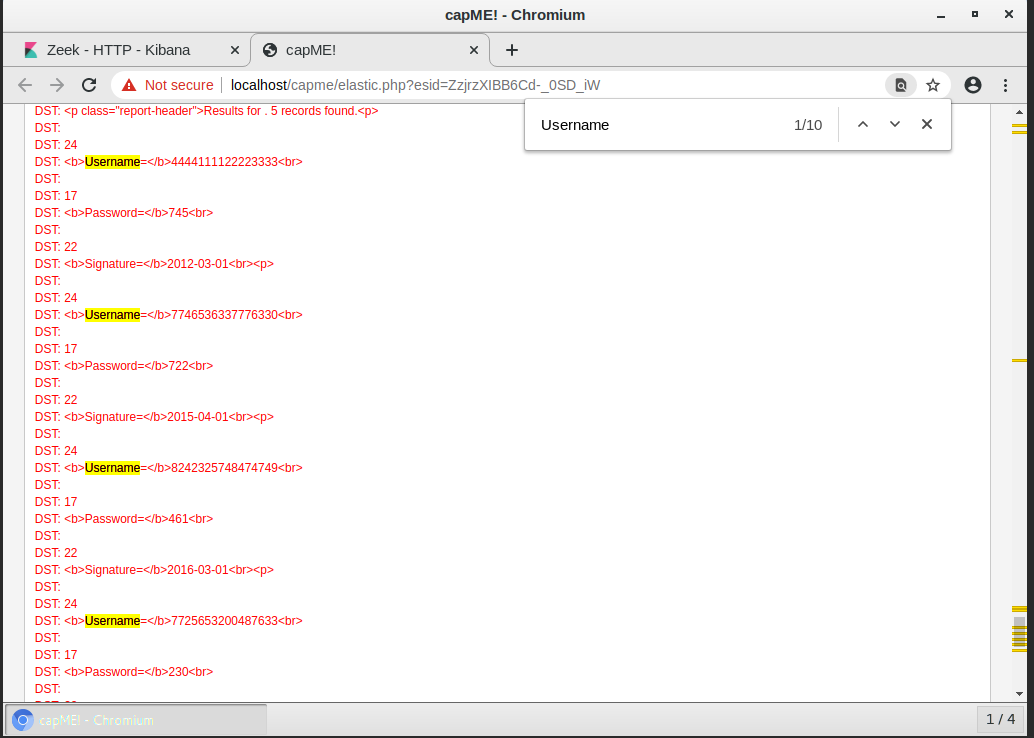
\includegraphics[width=0.95\linewidth]{img/capME.png}
    \caption{Transcripción en capME! con los datos de tarjetas obtenidos mediante inyección SQL.}
\end{figure}
\par{\sloppy\textbf{¿Qué puede ver más adelante en la transcripción en cuanto a nombres de usuario?}\par}
En la transcripción aparecen números de tarjetas bajo la etiqueta Username, códigos de verificación como Password y fechas de vencimiento como Signature. No son credenciales de usuarios, sino datos de tarjetas extraídos.

\par{\sloppy\textbf{Dé algunos ejemplos de un nombre de usuario, contraseña y firma que se exfiltró.}\par}
Ejemplos de la captura, usando sus etiquetas:
\begin{itemize}[itemsep=2pt]
    \item Username: \texttt{4444111122223333}; Password: \texttt{745}; Signature: \texttt{2012-03-01}.
    \item Username: \texttt{774653633776330}; Password: \texttt{722}; Signature: \texttt{2015-04-01}.
\end{itemize}


\clearpage
\subsection{Exfiltración mediante DNS}
Se revisaron los registros DNS de junio de 2020 y se filtraron las consultas relacionadas con \texttt{example.com} para decodificar sus subdominios.
\captura{dns.png}{Panel DNS de Kibana: 22 registros y puerto de destino 53.}
\captura{dnsQuery.png}{Consultas DNS con cadenas hexadecimales y opción de exportación.}

\clearpage
\captura{queryRara.png}{Cuatro consultas con subdominios hexadecimales filtradas por example.com.}
\captura{ips.png}{Detalle de una consulta DNS: dirección IP de origen y código SERVFAIL.}
\captura{ipscompletas.png}{Direcciones IP del cliente y del servidor DNS para las cuatro consultas filtradas.}
\par{\sloppy\textbf{Registre las direcciones IP del cliente y servidor DNS.}\par}
Cliente DNS: \texttt{192.168.0.11}. Servidor DNS: \texttt{209.165.200.235}.

\clearpage
\captura{hexaDecodificado.png}{Decodificación de las cadenas hexadecimales con \texttt{xxd -r -p}.}
\par{\sloppy\textbf{¿Los subdominios de las consultas DNS eran nombres legítimos? Si no, ¿cuál es el texto?}\par}
No eran nombres convencionales: contenían fragmentos de un documento codificados en hexadecimal. El texto recuperado es:
\begin{quote}\small
CONFIDENTIAL DOCUMENT\\
DO NOT SHARE\\
This document contains information about the last security breach.
\end{quote}

\par{\sloppy\textbf{¿Qué implica este resultado sobre esta respuesta DNS en particular? ¿Cuál es el mayor significado?}\par}
Los datos confidenciales viajaban dentro de las consultas DNS, lo que evidencia su uso como canal de exfiltración. El código \texttt{SERVFAIL} mostrado no demuestra que los datos hayan llegado a un servidor controlado por el atacante.

\par{\sloppy\textbf{¿Qué puede haber creado estas consultas DNS codificadas y por qué se seleccionó DNS como medio para exfiltrar datos?}\par}
Podría haberlas generado un malware o un script que divide y codifica el archivo. DNS suele estar permitido en la red, por lo que puede utilizarse para intentar sacar información entre consultas habituales.

\clearpage
\section{Laboratorio 27.2.14: análisis de cinco tuplas}
Las cinco tuplas corresponden a las direcciones IP y los puertos de origen y destino, junto con el protocolo utilizado. Se investigará qué ocurrió con el archivo \texttt{confidential.txt}.
\subsection{Revisión de alertas en Sguil}
\captura{sguil.png}{Alerta 5.1 en Sguil: respuesta con privilegios root y datos de la conexión TCP.}
\captura{servidoratacado.png}{Transcripción de comandos remotos y modificación del archivo /etc/passwd.}
\par{\sloppy\textbf{¿Qué tipo de transacciones ocurrieron entre el cliente y el servidor en este ataque?}\par}
Se intercambiaron comandos de una consola remota y sus respuestas mediante TCP. El atacante consultó \texttt{/etc/passwd} y agregó la cuenta \texttt{myroot} con UID 0, otorgándole privilegios de superusuario.
\clearpage

\subsection{Análisis del flujo TCP en Wireshark}
\captura{tcpstream.png}{Flujo TCP con comandos del atacante en rojo y respuestas del servidor en azul.}
\par{\sloppy\textbf{¿Qué observó? ¿Qué indican los colores de texto rojo y azul?}\par}
Se observa una consola remota sin cifrado. En esta captura, el rojo identifica los comandos enviados por el cliente atacante y el azul las respuestas del servidor.

\captura{whoiam.png}{Ejecución de whoami, información de red y lectura de /etc/shadow.}
\par{\sloppy\textbf{El atacante emite el comando \texttt{whoami} en el objetivo. ¿Qué muestra esto sobre el rol de atacante en el equipo de destino?}\par}
La respuesta es \texttt{root}: el atacante ejecutaba comandos con privilegios de superusuario.

\par{\sloppy\textbf{¿Qué tipo de datos ha estado leyendo el agente de amenaza?}\par}
Información del equipo y de la red, cuentas de usuarios en \texttt{/etc/passwd} y hashes de contraseñas en \texttt{/etc/shadow}.

\clearpage
\subsection{Investigación de FTP y archivos en Kibana}
Se revisaron los registros FTP y los archivos transferidos durante junio de 2020.
\captura{ftpentradas.png}{Entradas FTP con las direcciones IP, los puertos y la marca de tiempo.}
\par{\sloppy\textbf{¿Cuáles son las direcciones IP y los números de puerto de origen y de destino para el tráfico FTP?}\par}
Origen: \texttt{192.168.0.11:52776}. Destino: \texttt{209.165.200.235:21}. Corresponden a la conexión de control FTP sobre TCP.

\captura{credencialesatacante.png}{Transcripción FTP con autenticación y comando STOR para confidential.txt.}
\par{\sloppy\textbf{¿Cuáles son las credenciales de usuario para acceder al sitio FTP?}\par}
Usuario: \texttt{analyst}. Contraseña: \texttt{cyberops}. Ambas se transmiten en texto claro.

\clearpage
\captura{archivos.png}{Tipos MIME registrados en el panel de archivos.}
\par{\sloppy\textbf{¿Cuáles son los diferentes tipos de archivos? Mire la sección Tipo MIME.}\par}
\texttt{text/plain}, \texttt{image/jpeg}, \texttt{image/png}, \texttt{text/html}, \texttt{image/gif} e \texttt{image/x-icon}.

\captura{origenarchivos.png}{Orígenes de los archivos: HTTP y FTP\_DATA.}
\par{\sloppy\textbf{¿Cuáles son los orígenes de archivos enumerados?}\par}
HTTP (22 archivos) y FTP\_DATA (1 archivo).

\clearpage
\captura{MIME.png}{Tipo MIME y direcciones IP del archivo transferido mediante FTP.}
\par{\sloppy\textbf{¿Cuál es el tipo MIME, la dirección IP de origen y destino asociado con la transferencia de los datos FTP? ¿Cuándo ocurrió esta transferencia?}\par}
Tipo: \texttt{text/plain}. Origen: \texttt{192.168.0.11}. Destino: \texttt{209.165.200.235}. El registro FTP asociado muestra el 11 de junio de 2020 a las 03:53:09.086, según Kibana.

\par{\sloppy\textbf{¿Cuál es el contenido de texto del archivo que se transfirió mediante FTP?}\par}
Las capturas identifican el archivo \texttt{confidential.txt}, pero no muestran su contenido. Falta revisar la transcripción de FTP\_DATA para recuperarlo.

\par{\sloppy\textbf{Con toda la información recopilada hasta ahora, ¿cuál es su recomendación para detener nuevos accesos no autorizados?}\par}
Aislar el equipo comprometido, eliminar la cuenta \texttt{myroot}, cambiar las credenciales expuestas y corregir la vulnerabilidad. Restringir los accesos y reemplazar FTP por SFTP.

\clearpage
\section{Conclusión}
El análisis con Kibana, Sguil y Wireshark permitió identificar una inyección SQL, datos ocultos en consultas DNS y accesos con privilegios de administrador. La correlación de registros y tráfico facilitó reconstruir las acciones observadas y mostró la importancia de proteger las credenciales, restringir los accesos y monitorear la red.
\end{document}
